\documentclass[12pt]{article}
\usepackage{verbatim}
\usepackage[dvips]{epsfig}
\usepackage{color}
\usepackage{url}
\usepackage[colorlinks=true]{hyperref}

\begin{document}

\section*{GENESIS: Documentation}

{\bf Related Documentation:}
% start: userdocs-tag-replace-items related-do-nothing
% end: userdocs-tag-replace-items related-do-nothing

\section*{De Schutter: Purkinje Cell Model}

\begin{figure}[h]
\centering
   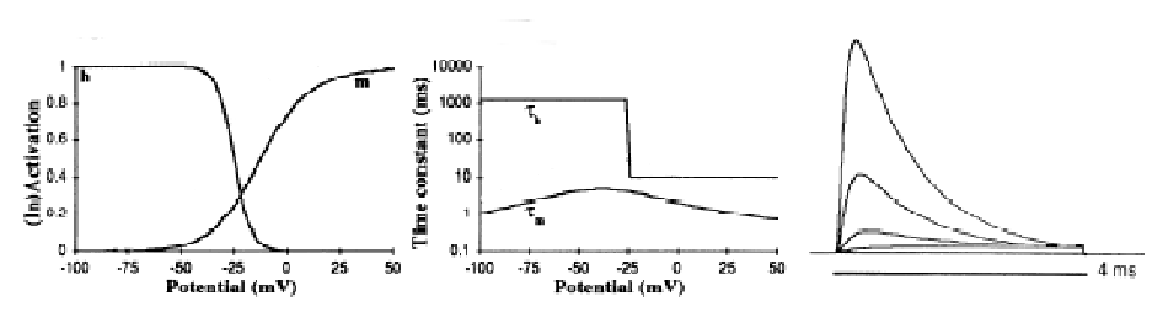
\includegraphics[scale=0.75]{figures/DS1.2E1.eps}
   \caption{Activation and inactivation properties of the delayed rectifier current (Kdr, ---) in the model. Seady-state activation and inactivation vs. voltage are plotted at the {\em left}, the time constants of activation and inactivation($\tau_m$ and $\tau_h$) vs. voltage in the {\em middle} (Note: Semilogarithmic scale), and a simulation of representative voltage-clamp currents at the {\em right}, obtained from a spherical cell and assuming a complete block of all other channels.  The voltage clamps simulate steps from a holding potential of -110 to -70\,mV up to 0\,mV in 10\,mV increments. The voltage-clamp current amplitude has been scaled arbitrarily because we mainly wanted to demonstrate the current kinetics.}
   \label{fig:DS1.2E}
\end{figure}

\subsection*{Delayed Rectifier (Kdr)}

The Purkinje cell delayed rectifier (Kdr) is responsible for the repolarization of somatic action potentials. Whole-cell voltage-clamp recordings (Fig. 9 in\,\cite{Hirano:1989uq}) and patch-clamp recordings (Fig. 9 in\,\cite{Gahwiler:1989fk}) of the Kdr current are available but incomplete. The $I-V$ relations of the currents in both reports are very similar. In the current model we have used the published equations for Kdr current in bullfrog sympathetic ganglion cells\,\cite{Yamada-W:1989bs} because both the $I-V$ curve and the steady-state inactivation (Fig. 2E) of the bullfrog data are comparable with the data from\,\cite{Hirano:1989uq}.

\bibliographystyle{plain}
\bibliography{../tex/bib/g3-refs}

\end{document}
